\section{Mote Harness}

In order to guarantee that both sender and receiver will not move during experiments a mote harness was developed and laser cut out of acrylic.
The mote snaps into the harness so that the axis of rotation goes through the middle of the PCB antenna which then allows rotation in 5$^\circ$ steps.
Furthermore, the distance between two harnesses can be adjusted in 5mm steps using laser-cut wooden distance bars.
Figure~\ref{fig:harness_picture} shows the harness with a mote on a distance bar and for better functional understanding a top view vector drawing of the rotation dish is shown in Figure~\ref{fig:harness_vector}.

\begin{figure}[ht]
	\subfigure[Harness with mote on a distance bar.] {
		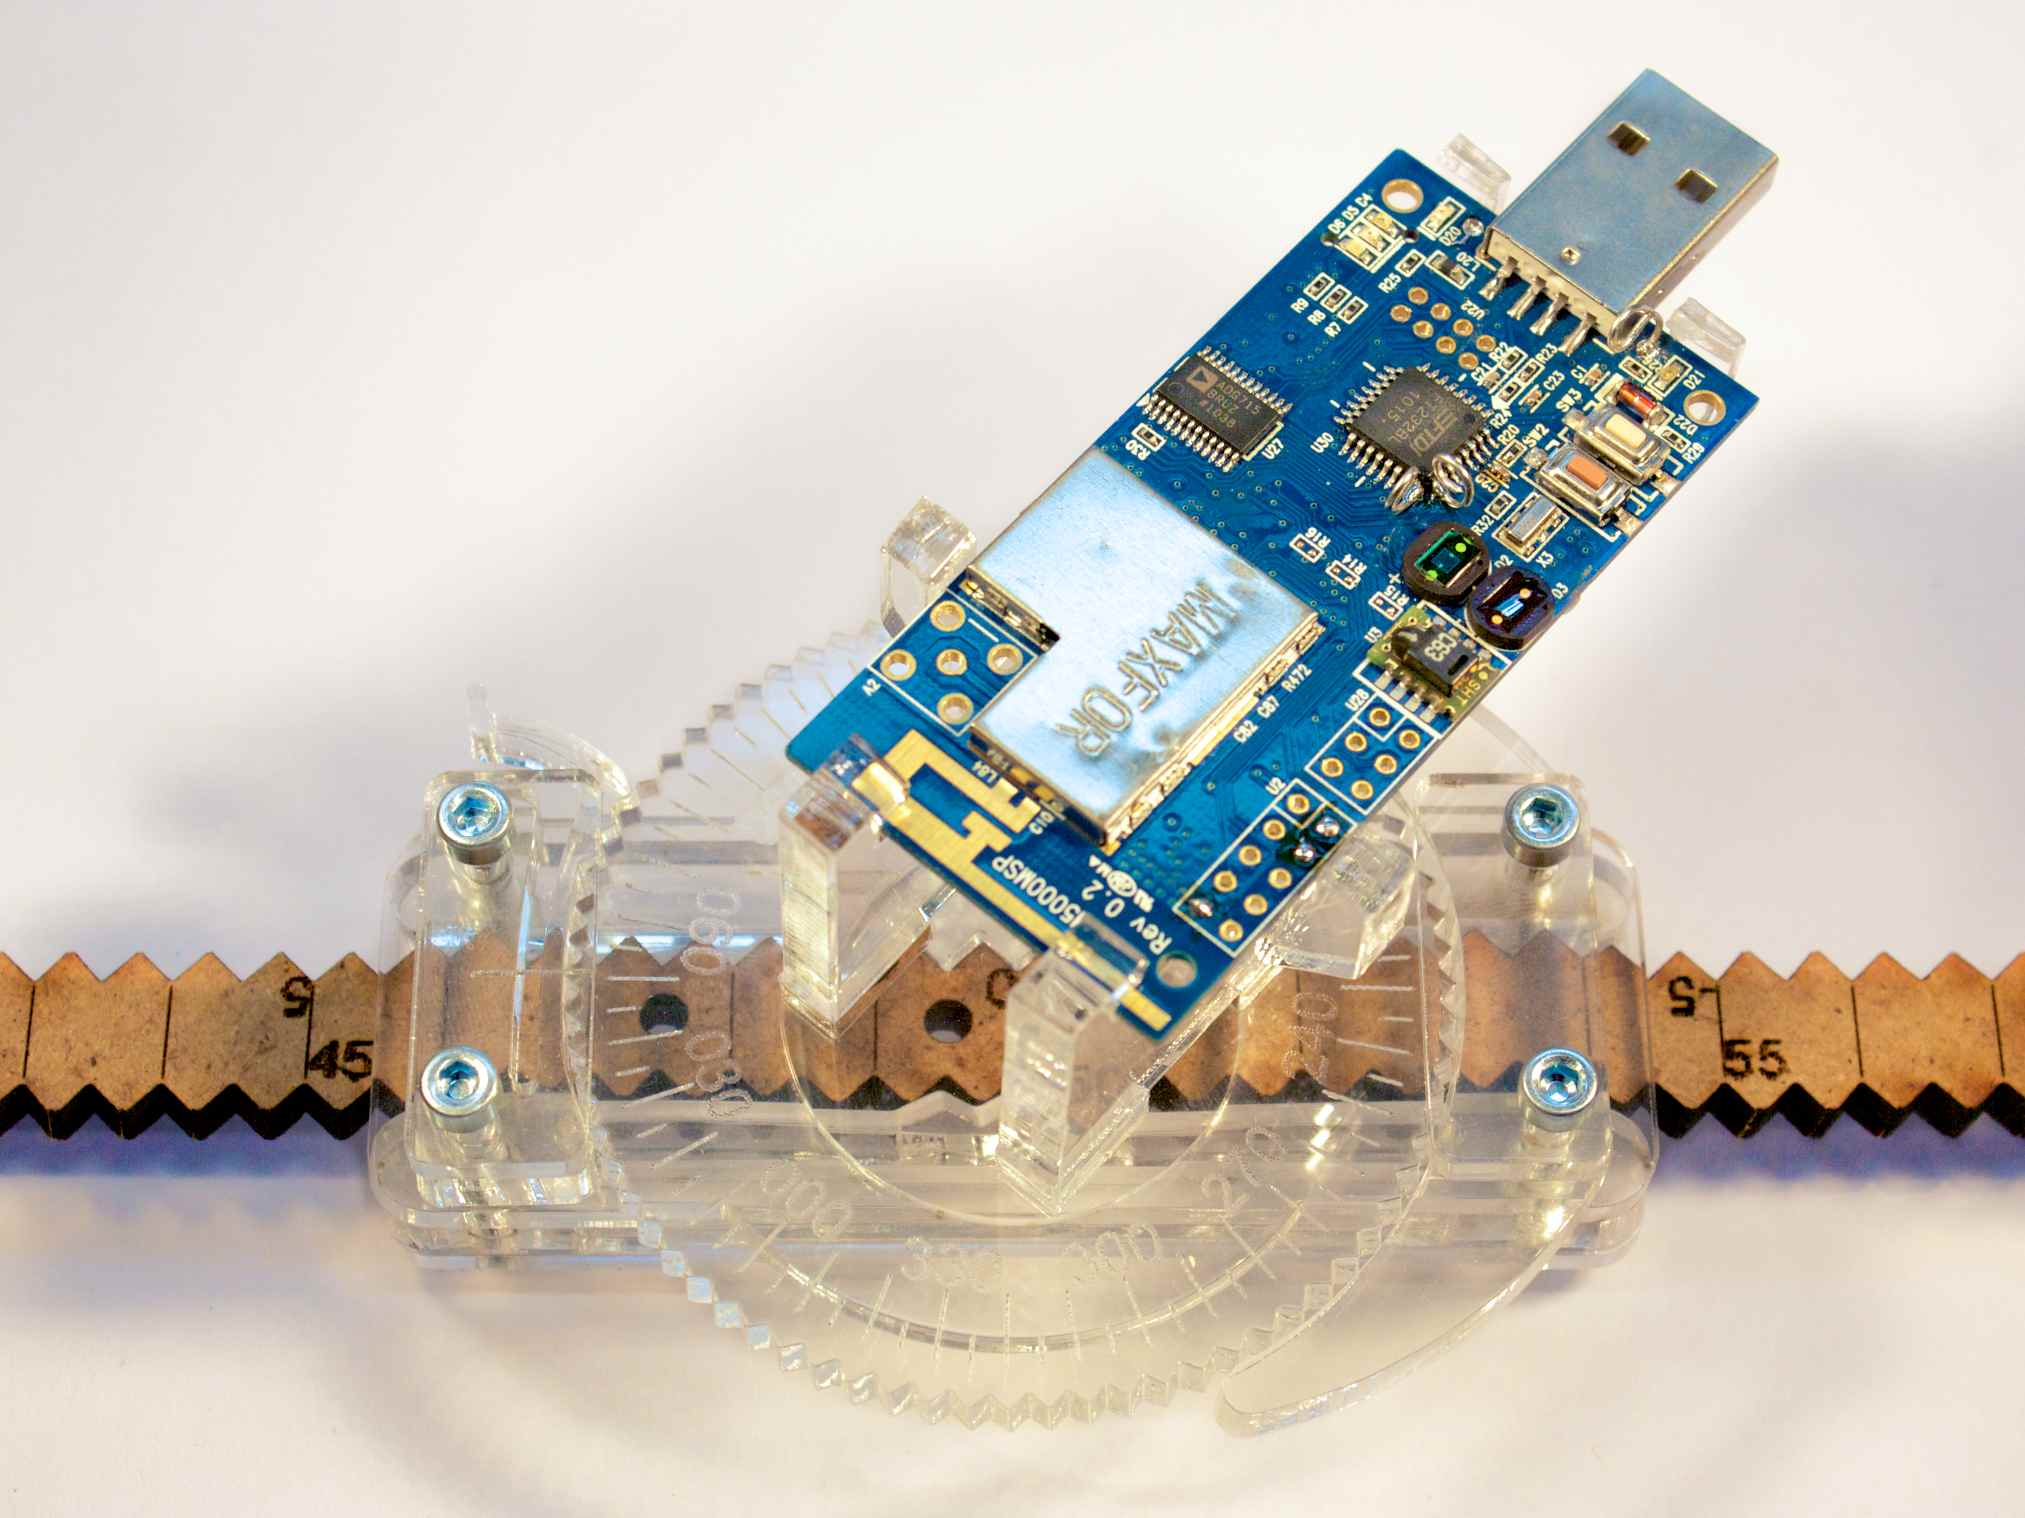
\includegraphics[width=0.5\columnwidth]{figures/harness_picture}
		\label{fig:harness_picture}
	}
	\subfigure[Vector drawing of the rotation disc.] {
		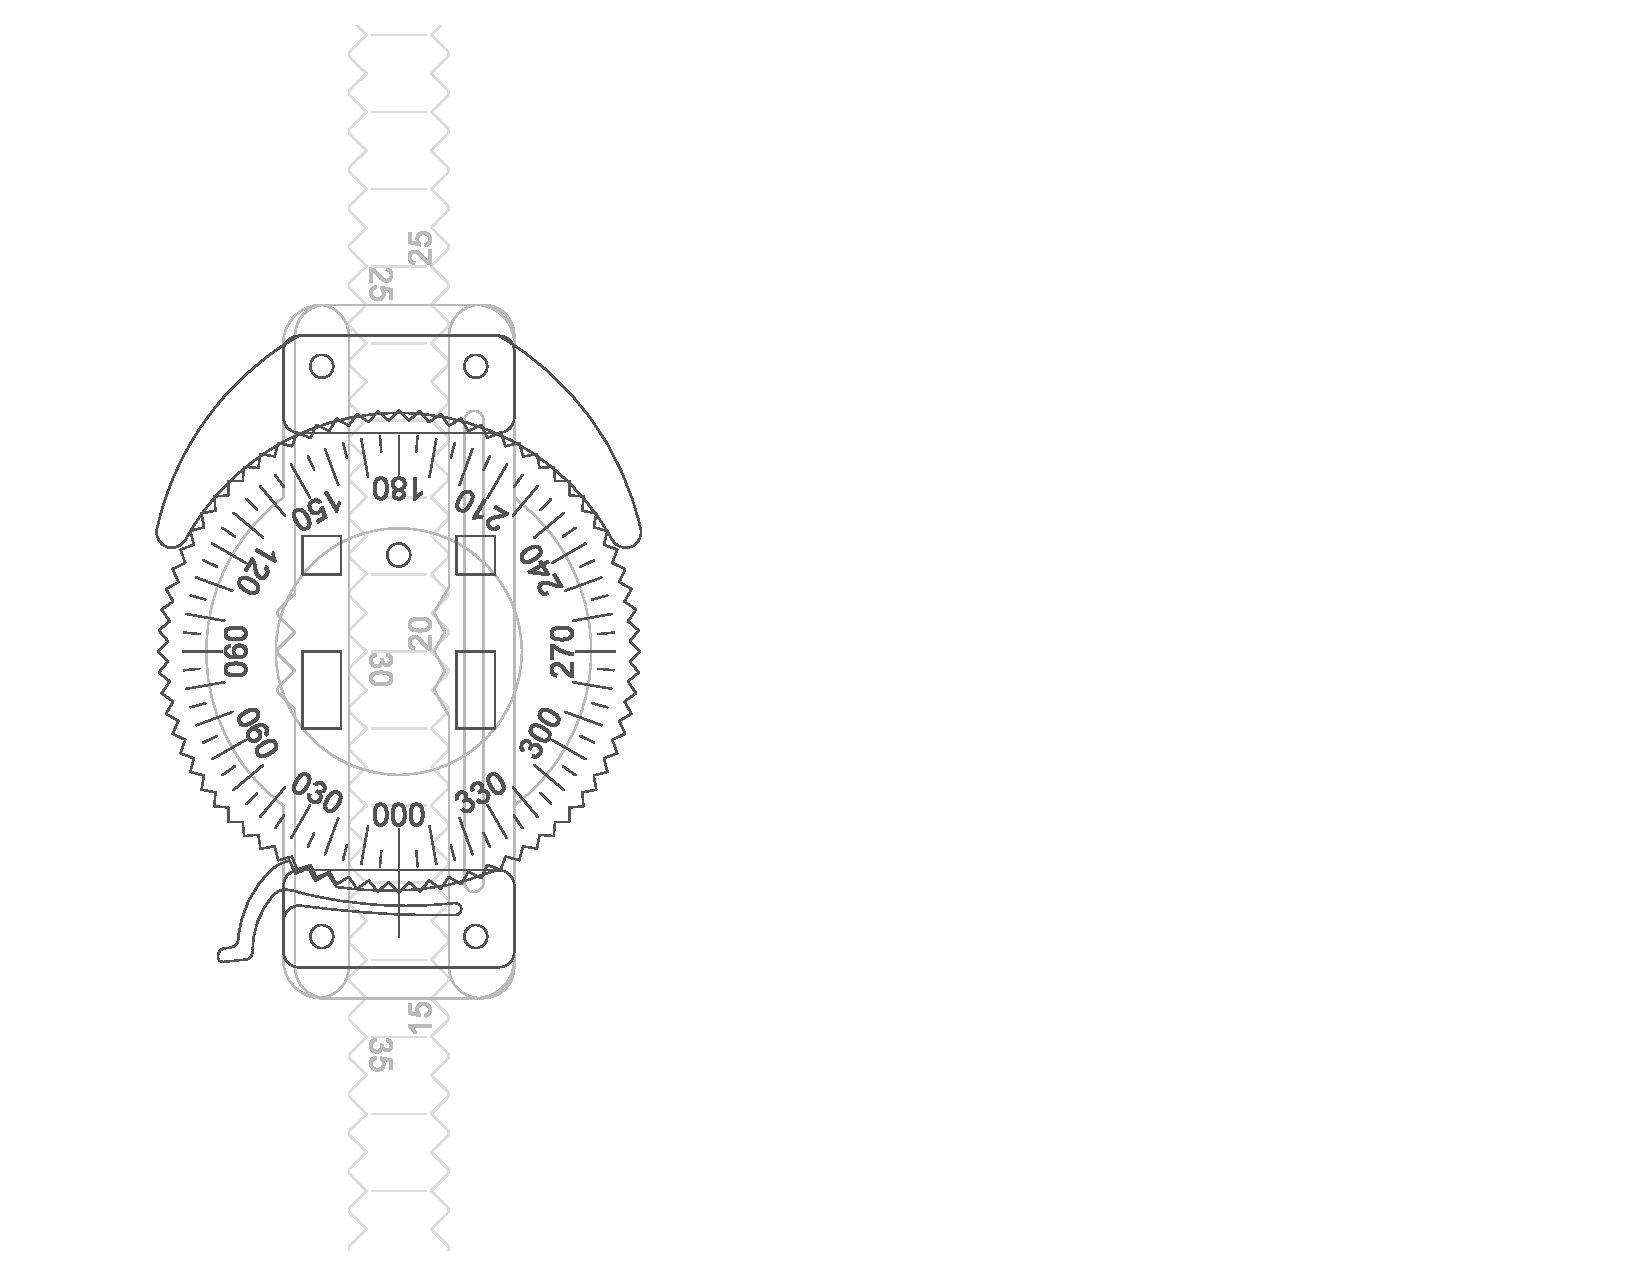
\includegraphics[trim = 20mm 40mm 140mm 45mm, clip, width=0.5\columnwidth, angle=90, scale=0.75]{figures/harness_vector_bar_2}
		\label{fig:harness_vector}
	}
	\caption{The mote harness allows precise positioning of motes.}
	\label{fig:8mote_bit_errors_simulation}
\end{figure}


